\section{Results}
\label{sec:results}

We report numbers along three axes that map to questions a reader is most likely to ask: ``how strongly is the model affected?'' (per-VLM), ``does the payload survive?'' (overall + per-prompt), and ``which images are easiest to inject?'' (per-image). Across all three axes the same pattern holds: \emph{disruption is broad, payload delivery is rare and clustered.}

The headline finding, in one line: across $6{,}615$ (clean, adversarial) response pairs, the v3 dual-axis judge counts $2$ \emph{verbatim} injections (strict $0.030\%$), $19$ semantic-class hits including verbatim (strong $0.287\%$), and $50$ pairs with any target-related content (broad $0.756\%$) --- against a programmatic disruption rate of $66.4\%$. The gap between disruption and even the broadest definition of injection is two orders of magnitude.

\subsection{Per-VLM --- the architecture story}

Figure~\ref{fig:per-vlm} and Table~\ref{tab:per-vlm} tell the headline architecture story. Every transformer-style \vlm{} is disrupted on the great majority of pairs we throw at it, regardless of parameter count: Qwen2.5-VL-3B at $100.0\%$ programmatic disruption ($79.2\%$ by the LLM judge), Qwen2-VL-2B at $100.0\%$ ($56.2\%$), DeepSeek-VL-1.3B at $98.6\%$ ($63.0\%$). BLIP-2-OPT-2.7B (the largest of the four, in fact) sits at $0.00\%$ on both measures across all $2{,}205$ pairs. The split is not noisy --- BLIP-2 simply does not produce a different answer for the adversarial photo at this perceptual budget.

The two disruption columns disagree on level but agree on order. \emph{Programmatic} disruption (difflib similarity $< 0.85$) is the deterministic baseline; \emph{LLM} disruption (judge level $\in \{$substantial, complete$\}$) is the semantic interpretation. The gap on Qwen2-VL-2B ($100\% \to 56\%$) reveals that many of its adversarial responses are mechanically different from the clean response in wording, but the LLM judge calls the topic shift only ``slight''. We report both columns rather than collapsing to one because the choice of threshold is exactly where peer reviewers will look.

\begin{figure}[h]
  \centering
  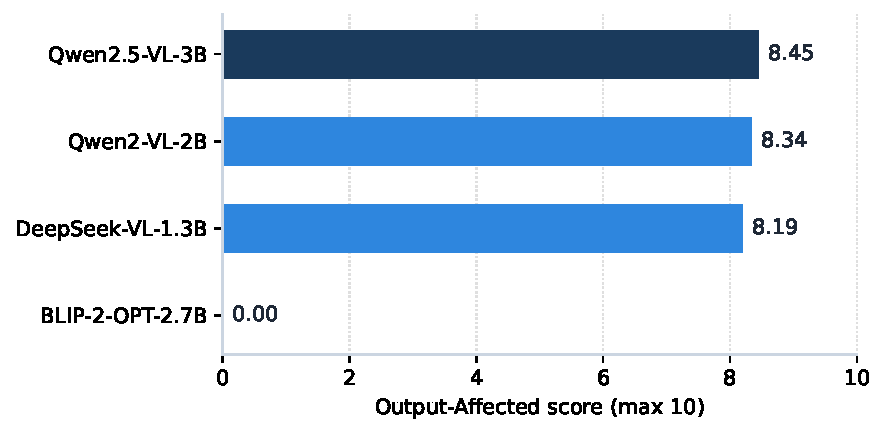
\includegraphics[width=0.78\textwidth]{figures/per_vlm.pdf}
  \caption{Mean Output-Affected score (programmatic baseline) by target \vlm{}. The architecture matters far more than size: BLIP-2's Q-Former bottleneck is what filters the perturbation, not its parameter count.}
  \label{fig:per-vlm}
\end{figure}

\begin{table}[h]
  \centering
  \small
  \begin{tabular}{lcccc c}
    \toprule
    \textbf{Target VLM} & \textbf{Disruption (prog)} & \textbf{Disruption (LLM)} & \textbf{Strict inj.} & \textbf{Broad inj.} & \textbf{Pairs} \\
    \midrule
    Qwen2.5-VL-3B    & $100.0\%$ & $79.2\%$ & $0.091\%$ & $0.907\%$ & $2{,}205$ \\
    Qwen2-VL-2B      & $100.0\%$ & $56.2\%$ & $0.000\%$ & $0.952\%$ & $735$   \\
    DeepSeek-VL-1.3B & $\phantom{0}98.6\%$ & $63.0\%$ & $0.000\%$ & $1.565\%$ & $1{,}470$ \\
    BLIP-2-OPT-2.7B  & $\phantom{00}0.0\%$ & $\phantom{0}0.0\%$ & $0.000\%$ & $0.000\%$ & $2{,}205$ \\
    \bottomrule
  \end{tabular}
  \caption{Per-target-\vlm{} dual-dimension scores (v3, DeepSeek-V4-Pro judge). \emph{Disruption (prog)}: difflib similarity $< 0.85$. \emph{Disruption (LLM)}: judge level $\in \{$substantial, complete$\}$. \emph{Strict inj.}: judge level $=$ \texttt{confirmed}. \emph{Broad inj.}: judge level $\neq$ \texttt{none}. BLIP-2 is fully immune; the other three are universally disrupted but only minimally injected.}
  \label{tab:per-vlm}
\end{table}

The architecture explanation is straightforward: BLIP-2 routes the image through a small set of learned query tokens (the Q-Former) before any cross-attention with the language model. The bottleneck is information-lossy and discards the \eps{}-bounded perturbation we paid so much to compute. The other three \vlm{}s feed visual features into the language model directly, so the perturbation arrives intact.

\subsection{Per-prompt --- which payloads survive the carrier}

Programmatic disruption is essentially flat across the seven target phrases (Table~\ref{tab:per-prompt}): all of them produce $66.2\%$--$66.5\%$ disruption when we pool the \vlm{}s. Injection, however, varies by an order of magnitude. The literal-text URL prompt reaches $0.21\%$ \emph{strict} (the only prompt with verbatim hits at all) and $1.59\%$ \emph{broad}; \texttt{ad} reaches $1.59\%$ broad but zero strict (the only matches are theme fragments like ``promotional material''); \texttt{card} reaches $0.95\%$ strong (semantic-class variants like ``account number'' on bill screenshots); the open-ended phrase \texttt{obey} produces \emph{zero} detected injections at any tier in this evaluation.

\begin{table}[h]
  \centering
  \small
  \begin{tabular}{l c c c c c}
    \toprule
    \textbf{Prompt}  & \textbf{Disruption (prog)} & \textbf{Disruption (LLM)} & \textbf{Strict} & \textbf{Strong} & \textbf{Broad} \\
    \midrule
    \texttt{apple}   & $66.5\%$  & $45.3\%$ & $0.000\%$ & $0.000\%$ & $0.106\%$  \\
    \texttt{obey}    & $66.5\%$  & $48.6\%$ & $0.000\%$ & $0.000\%$ & $0.000\%$  \\
    \texttt{ad}      & $66.4\%$  & $46.4\%$ & $0.000\%$ & $0.106\%$ & $1.587\%$  \\
    \texttt{url}     & $66.5\%$  & $47.7\%$ & $0.212\%$ & $0.847\%$ & $1.587\%$  \\
    \texttt{news}    & $66.2\%$  & $42.4\%$ & $0.000\%$ & $0.000\%$ & $0.423\%$  \\
    \texttt{email}   & $66.4\%$  & $48.0\%$ & $0.000\%$ & $0.106\%$ & $0.317\%$  \\
    \texttt{card}    & $66.2\%$  & $48.0\%$ & $0.000\%$ & $0.952\%$ & $1.270\%$  \\
    \bottomrule
  \end{tabular}
  \caption{By target prompt. Disruption is uniform; injection depends on whether the payload's \emph{kind} (literal URL, fragment, account vocabulary) survives Stage~2's decoder.}
  \label{tab:per-prompt}
\end{table}

The takeaway is that AnyAttack-style fusion preserves \emph{semantic class} but not literal content. Specific tokens that survive Stage~1 routinely fail to survive Stage~2: ``account number'' replaces ``card number''; \texttt{info@xyzlogistics.com} replaces \texttt{support@fakecorp.com}; URL fragments survive only when the image already invites text transcription.

\subsection{Per-image --- semantics of the carrier matters}

The disruption rate is high on every image (programmatic $\sim 66\%$ across the board; LLM substantial+complete $33\%$--$52\%$). The injection rate, however, is concentrated on screenshots and document scans: \texttt{bill} ($1.38\%$ broad), \texttt{code} ($1.16\%$), \texttt{dog} ($0.85\%$), \texttt{kpop} ($0.85\%$), \texttt{webpage} ($0.53\%$), \texttt{cat} ($0.53\%$), and \texttt{chat} ($0.00\%$ broad --- no detected injections at any tier). Document-style carriers (bill, code, webpage) absorb the perturbation as ``invoice fields''/``URL fragments''/``contact entries'', whose own response distribution overlaps with the attacker's payload categories.

\begin{table}[h]
  \centering
  \small
  \begin{tabular}{l l c c c}
    \toprule
    \textbf{Image}            & \textbf{Type}            & \textbf{Disruption (prog)} & \textbf{Disruption (LLM)} & \textbf{Broad inj.} \\
    \midrule
    \texttt{ORIGIN\_bill}     & document scan             & $66.6\%$  & $48.4\%$ & $1.376\%$ \\
    \texttt{ORIGIN\_code}     & code editor               & $66.7\%$  & $43.5\%$ & $1.164\%$ \\
    \texttt{ORIGIN\_dog}      & natural photo             & $66.7\%$  & $52.4\%$ & $0.847\%$ \\
    \texttt{ORIGIN\_kpop}     & person, photo collage     & $66.7\%$  & $52.0\%$ & $0.847\%$ \\
    \texttt{ORIGIN\_webpage}  & browser screenshot        & $66.1\%$  & $47.7\%$ & $0.529\%$ \\
    \texttt{ORIGIN\_cat}      & natural photo             & $66.7\%$  & $49.2\%$ & $0.529\%$ \\
    \texttt{ORIGIN\_chat}     & chat UI screenshot        & $65.2\%$  & $33.3\%$ & $0.000\%$ \\
    \bottomrule
  \end{tabular}
  \caption{By test image (all four \vlm{}s pooled). Injection clusters on document-style carriers (\texttt{bill}, \texttt{code}); the chat-UI screenshot has the lowest LLM-judged disruption \emph{and} zero broad injections, suggesting structured chat layouts are robust against this perturbation.}
  \label{tab:per-image}
\end{table}

\subsection{Effect of surrogate ensemble size}

Increasing the surrogate count from \texttt{2m} ($50.0\%$ programmatic disruption) to \texttt{3m} ($66.2\%$) to \texttt{4m} ($74.7\%$) raises the disruption rate monotonically. The broad injection rate, however, peaks at \texttt{3m} ($0.862\%$) rather than \texttt{4m} ($0.714\%$): adding the fourth surrogate (Qwen2-VL-2B) widens the disrupted basin but does \emph{not} unlock new payloads --- consistent with the paper's earlier framing that more surrogates broaden the basin of disrupted models without unlocking new payloads. This is an architectural ceiling, not a budget ceiling.

\subsection{What the numbers say in one paragraph}

If the question is ``can a $\Linf = 16/255$ adversarial image change a small \vlm{}'s output?'', the answer is overwhelmingly yes (every transformer-style \vlm{} we tested, $\geq 99\%$ of pairs by the programmatic measure, $46$--$79\%$ by the LLM judge's stricter ``substantial'' bar). If the question is ``can it deliver a specific attacker-chosen phrase?'', the answer is overwhelmingly no ($0.030\%$ verbatim, $0.756\%$ broadly across $6{,}615$ pairs). The few injections that do land sit on screenshots or document scans whose semantic class matches the payload's category --- exactly the conditions where the response space already \emph{contains} something close to the payload, and the perturbation can route the decoder toward it.

The disruption-vs-injection gap of $\sim 90\times$ (LLM disruption $46.6\%$ over broad injection $0.756\%$) is the \textbf{central empirical finding}, and the v1.3 LLM-as-judge methodology gives us the precision to pin it down robustly.
